\chapter{绪论}

高性能计算技术广泛应用于能源、环境、气候、医疗、生物等国家重点行业,
是提升国家军事、经济、科技、安全等方面实力的重要工具,
具有十分重大的战略意义,其发展水平已经成为国家综合实力的体现之一。
过去三十年, 计算能力呈指数增长。
2008年,高性能计算机的运算能力达到P级($10^{15}$ flops),
2017年11月TOP500\upcite{top500}排名第一的"神威$\cdot$太湖之光"高性能计算机性能已经
接近100P($93.015\times10^{15}$ flops),
现在,世界各超算强国都在积极研发E级($10^{18}$ flops)高性能计算机。
%% 预计第一台E级系统将于2020年问世。
然而,E级高性能计算机的研制正面临着巨大的挑战
\upcite{廖湘科2016新型高性能计算系统与技术}。
随着系统规模的增加,无论是能耗、通信、编程还是存储和可靠性,
仅依靠已有的计算模型和大规模并行框架并不能使系统性能大幅度增长。
如,天河二号高性能计算机运算能力为$33.86\times10^{15}$ flops,能耗为17.8MW。
若采用与天和二号同样的技术,E级计算机的能耗保守估计约534MW,
这大大超出了所能承受的范围。
同时,大数据、云计算等业务的持续增长,也对传统高性能计算提出新的挑战和需求。
美国、日本、德国等国均对E级高性能计算系统的研制做出了相应的规划和部署,
Intel、Nvidia、IBM、Cray等企业已经开始关键技术的攻关。
因此,E级高性能计算机的研制是一个竞争极为激烈的领域。

\section{研究背景和意义}
本节介绍论文的研究背景,首先介绍了当前主要高性能计算机系统的基本情况,
然后阐述了高性能互连网络对于高性能计算机系统的重要性并给出互连网络设计
中需要考虑的主要因素,
最后介绍高性能互联网络的相关研究现状。

\subsection{高性能计算机}

\subsubsection{神威$\cdot$太湖之光}
“神威$\cdot$太湖之光”高性能计算机系统\upcite{Taihulight},
峰值运算速度$93.015\times10^{15}$ flops,在2017年11月与2018年6月的
TOP500排名中分别位列第一与第二。
“神威$\cdot$ 太湖之光”采用异构体系结构,
其计算节点使用国产申威26010(SW26010)异构众核处理器,
该处理器由260个处理单元构成,单处理器性能超过$3\times10^{12}$ flops。
“神威$\cdot$ 太湖之光”的系统构成为:
每8个计算节点通过PCB 板相连接,
每256个计算节点组成一个超级节点,
每4个超级节点组成一个机柜,
全系统包括共计40个机柜40960个计算节点。
“神威$\cdot$ 太湖之光” 采用三层不同层次的互连网络。
顶层是中央交换网络,负责不同超级节点间的数据交换。
中间一层是超级节点网络,每个超级节点内部256个计算节点全互连。
最底层是资源共享网络,提供服务和连接共享资源给超级节点。
网络二分带宽为$7\times10^{12}$ Bps, 直径为7,功耗15.37MW。

\subsubsection{天河二号}
天河系列高性能计算机曾经七次占据TOP500排名榜首。
天河二号\upcite{Liao2015}峰值运算速度$33.86\times10^{15}$ flops,
在2017年11月与2018年6月的TOP500排名中分别位列第二与第四。
天河二号同样采用异构体系结构,其计算节点由2个
Intel Xeon E5-2600处理器和3个Intel Xeon Phi加速器组成。
%% 其峰值性能为$3.432\times10^{12}$ flops。
天河二号的系统构成为:
每2个计算节点封到一个计算板,
每16个计算板与1个交换板、1个控制板组成一个计算框架,
每4个计算框架组成一个机柜,
全系统最多包括144个机柜18432个计算与I/O节点。
天河二号互连网络采用8-lane 24端口高阶路由芯片,
聚合带宽$5.376\times10^{12}$ bps。
%% FIXME I cannot understand the network structure 
天河二号互联网络采用三层胖树结构,
第一层结构中每32个计算节点连接在一块交换板上,
每个交换板是一个计算框架,
每四个计算框架组成一个机柜。
每个交换板是由6个24端口的芯片连接而成的两层胖树,
共引出36条光纤连接第二层的交换芯片。
第二层的交换芯片是24 端口的,
分别给12个端口连接第三层和第一层,
连接第一层的12个端口分别用来连接不同的12个计算框架,
也就是3 个机柜。
第三层实际上是个两层胖树结构,
由6 个24 端口的芯片连接而成的48 端口交换机。

\subsubsection{Piz Daint}
Piz Daint是欧洲最快的高性能计算机,由瑞士联邦理工学院投资建造,
峰值运算速度$19.590\times10^{15}$ flops,
在2017年11月与2018年6月的TOP500排名中分别位列第三与第六。
Piz Daint采用Cray XC50高性能计算机模型\upcite{crayxc50},
互连网络采用Dragonfly结构\upcite{dragonfly}。
Piz Daintde 系统构成为:
每4个计算节点组成一个计算板,
每16个计算板通过背板全互连成一个机架,
每3个机架组成一个机柜,
每2个机柜组成Dragonfly网络中的1个group结构。
每个group内的6个机架通过电缆全互连。
整个系统中的所有group通过光缆全互连。

\subsubsection{PRIMEHPC FX10}
PRIMEHPC FX10\upcite{primehpcfx10}是继“K computer”后,
Fujitsu公司推出的新一代高性能计算机,
其峰值性能可达$23.2\times10^{15}$ flops。
PRIMEHPC FX10采用低能耗SPARC64 IXfx处理器芯片,
整个系统规模最高可达1024个机柜,
含98304个计算节点和6144 个I/O节点,功耗约23MW。
PRIMEHPC FX10互连网络采用的是6D Mesh/Torus 结构,如图\ref{tofuto}所示,
%% FIXME tofu? 6Dmesh/torus?
以Tofu\upcite{tofu} 模块为单元进行XYZ三维连接。
Tofu模块内嵌ABC三维结构。
网络中X维链路和Y维链路连接各个机柜,
Z维链路和B维链路相连各个系统板。
A维链路和C维链路相连4个节点构成一个系统板。
Fujitsu公司正在研制新一代E级高性能计算机Post-FX10,
计划采用的互联结构为Tofu的升级版——Tofu 2\upcite{tofu2},
该系统不仅提升了CPU和网络的性能,
而且具备更高的封装性和更低的功耗以支持E级计算的规模。

%% FIXME is this figure necessary?
\begin{figure}[htp]
\centering
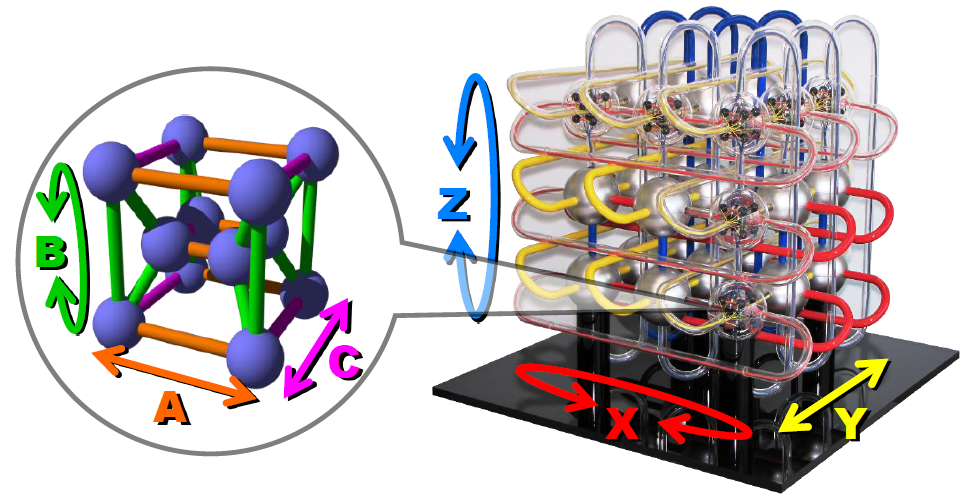
\includegraphics[width=.8\textwidth,height=.4\textwidth]{tofu.png}
\caption{Tofu模块和6D Mesh/Torus结构\upcite{tofu}}
\label{tofuto}
\end{figure}

\subsection{高性能互连网络}

E级高性能计算机系统的研制和应用面临巨大的挑战,
%% 对高性能互连网络来说则面临更大的挑战。
高性能互连子系统的设计则是其中最具挑战性的部分之一。
作为高性能计算机系统的重要组成部分,
互连网络的主要功能是完成计算节点、I/O节点之间的通信。
随着处理器性能按照摩尔定律提升、
计算系统规模的按照指数级增长,
互连网络越来越成为影响系统性能的主要因素\upcite{johnkim}。
高性能互连网络主要由四个重要部分构成:
拓扑结构,路由算法,拥塞控制以及物理器件。
拓扑结构决定了报文在网络中最短跳步数、
节点间可用的总路径数和二分带宽,
路由算法则决定了报文在网络中的实际跳步数。
物理器件主要指通过拓扑结构相连的封装在机柜内的路由器和物理链路。
实际高性能互连网络通信则是依靠路由算法和拥塞控制机制保证。
在高性能互连网络设计中需要考虑很多因素\upcite{duato2002interconnection},
主要包括:

\textbf{网络性能}。消息延迟和网络的吞吐率是网络性能的主要指标。
消息延迟是指消息在源节点开始发送的时间与目的节点接收消息的时间间隔。
消息延迟直接影响处理器和存储的使用。
吞吐率则是在单位时间内,网络所能传输最大的信息量。
因为成本开销等原因,网络容量是有限的,
一旦饱和网络不会再传输新注入的消息,
%% 这严重限制了系统的性能。
消息延迟与吞吐率与网络直径和链路容量紧密相关。

\textbf{灵活性和扩展性}。灵活性是指在扩大或者缩小规模的同时,
相应的带宽需求也按需求按比例增减,以保证性能不降低。
否则,带宽将成为系统瓶颈,降低系统效率。
扩展性指在物理器件约束下,在保证网络性能的前提下,
网络仍然能够支持的最大规模。

%% FIXME 应用负载?
\textbf{应用负载}。网络可以根据应用负载的不同将网络中的节点或者链路划分成多个子网,
使得不同应用负载之间互相不影响性能。同时,隔离不同的负载也可以提高安全性。

\textbf{物理封装和器件约束}。结合实际物理封装因素考虑
如何保持高性能互连网络拓扑本身的优良特性是设计高性能互连网络拓扑的重要问题。
物理封装有两个主要限制影响拓扑设计,一是缆线的长度和数量,二是芯片的带宽和引脚数。
随着光纤技术的发展,机柜内部因为距离较短采用电信号传输,
机柜之间则采用光纤保证长距离的通信质量。
随着系统规模的增大,机柜数增长,不仅缆线数量增加使得物理封装难度提高,
缆线长度也因此增加而造成网络延迟增加。
芯片的带宽和引脚数受限于芯片的面积,
在高阶路由器和光纤技术等器件发展不成熟时期,
互连网络受器件约束只能采用节点度数小,
网络直径大的拓扑结构,如经典的$k\textrm{-}ary$ $n\textrm{-}cube$结构。
随着工艺的进步,高阶路由器等器件的技术已成熟,
采用低直径网络拓扑结构成为高性能互连网络设计的主流趋势。
%% 除了此之外,简单性和可维护性都跟拓扑设计紧密相关的。
%% 一个好的高性能互连网络拓扑结构一定是易构造,易维护的。

\textbf{可靠性}。高性能互连网络是无损网络,
不支持丢包和重传。
因此,高性能互连网络的可靠性是保证网络传输的重要指标。
一旦有错误发生,网络中有多条可选路径保证传输不受影响。
%% FIXME? the sentence above
并且,在设计拓扑结构时必须将条链路或者节点发生故障的可能纳入考虑,
虑以保证网络可以容忍一定的故障率。

\textbf{成本能耗开销} 。随着系统规模的增加,
路由器数目和缆线数量的增加,都大大增加了成本和能耗的开销。
尤其,在能耗方面,若是随着规模的增加而线性增长,
将无法完成E级高性能计算机系统的开发。
因此,在设计网络拓扑结构时,成本能耗限制是起决定性影响的因素。

\subsection{研究现状和不足}

本节主要回顾国际上在高性能互连网络设计方面的相关工作。
自高性能计算机系统发展以来,在HPCA、ISCA、 SC、 ICS等高性能领域顶级会议上,
高性能互连网络一直都是热点研究方向。
Intel、Cray、IBM、Bull、Mellanox等公司以及
学术界许多研究小组都在关注和致力于开展
高性能互连网络的拓扑结构设计,路由算法及拥塞控制等方面的研究。

\subsubsection{拓扑结构相关研究}
在高性能计算机系统发展早期,
高性能计算机系统的互连网络大多数采用树形、
$k\textrm{-}ary$ $n\textrm{-}fly$蝶形等间接网络结构,
或$k\textrm{-}ary$ $n\textrm{-}cube$直接网络结构。
这些结构的特点都是使用端口数较小的交换机通过多级或者笛卡尔积的方式构建网络。

随着高阶路由器结构和光纤技术的发展,低直径网络拓扑结构开始成为
构造大规模高性能互连网络的可行方案。
2007年,Kim等人在ISCA会议上提出了使用高阶路由器搭建大规模
高性能互连网络的低直径拓扑结构Flattened Butterfly\upcite{Flattenedbutterfly},
用高阶路由器替代传统的低阶路由器,从而减少路由器数量并降低网络直径。
之后,该组在2008年的ISCA会议上提出新型
高性能互连网络拓扑结构Dragonfly\upcite{dragonfly},
在2009年的SC会议上提出可灵活配置的HyperX结构\upcite{hyperx},
不仅充分利用高阶路由器的特点还将光纤运用在拓扑结构的不同层次。
此后,采用低直径拓扑结构构建大规模高性能互连网络成为高性能互连网络的发展趋势,
Cray、IBM等大公司也开始使用高阶路由器搭建高性能计算系统,
如Cray公司的Cascade系统\upcite{cascade}和IBM的PERCS系统。

Koibuchi所在的研究小组在2012年的ISCA会议上提出了
使用高阶路由器搭建随机拓扑\upcite{acaserandom},
该拓扑不仅网络直径低,平均最短路径小,还可以支持任意的网络规模。
但是,随机拓扑在物理布局中,面临缆线长短不一,连线复杂等问题。
该研究组在2013年的HPCA会议上提出layout-conscious的随机拓扑结构\upcite{fsorandom},
根据实际物理降低缆线的长度减少系统构建的开销。
2015年的HPCA 会议上,他们小组提出在机柜上摆放自由光设备,
根据不同应用的负载,在随机拓扑上添加自由光链路以满足不同的链路需求。
2014年的SC会议上瑞士联邦理工的Besta和Hoefler利用代数图论的方法
构造出近似最优的低直径拓扑Slim Fly\upcite{slimfly}。
Slim Fly结构在不受路由器端口数限制的条件下,相比其他拓扑结构,
%% 到底是端口数受限,还是不受限?
不仅端口利用率高,还取得了更优的网络性能。
2015年SC会议上Kathareios等人提出一个性价比更高,
直径为2的拓扑结构OFT\upcite{costeffective2}。
在同样的成本开销下,OFT结构相比Slim Fly结构,拥有更好的可扩展性。

\subsubsection{路由算法相关研究}
高性能互连网络的路由算法是高性能互连网络的研究重点。
路由算法决定了拓扑结构的实际网络性能,
因此,即便拓扑结构具备优良的结构特性,
如果没有合适的路由算法,互连网络也无法发挥出优秀的性能。
当前,低直径拓扑结构成为构建大规模高性能互连网络的首选方案,
这也给路由算法设计带来了巨大挑战。
Jiang等人在2009年ISCA会议上对Dragonfly结构提出
间接自适应路由,通过本地链路间接反馈来解决全局链路的拥塞\upcite{indirect}问题。
随后,Garc\'ia等人分析出现有的自适应路由算法在解决
Dragonfly结构全局链路拥塞问题的同时引入了本地链路的拥塞,
提出了On-the-fly路由算法\upcite{On-the-Fly}解决全局和本地链路拥塞的问题。
由于On-the-fly路由算法采用自适应绕路路由,
如果采用虚通道隔离的方式避免死锁,
路由芯片需要增加虚通道数目,从而增加缓存资源和控制单元,
导致成本上升甚至超出芯片面积限制。
如果采用逃逸子网的方式避免死锁,
逃逸路径过长会严重影响网络性能。
因此,Garc\'ia 等人提出了OFAR-CM\upcite{OFAR-CM}、
RLM\upcite{Rlmolm}和OLM\upcite{Rlmolm}解决On-the-fly路由算法在死锁避免方面的问题,
减少虚通道数量并保证网络性能。
Won等人在2015年HPCA会议上提出了避免
Dragonfly远端拥塞的路由算法\upcite{ofc},
通过添加历史窗口观察正在链路上传输的报文以判断应该走最短路径还是非最短路径。

\subsubsection{拥塞控制相关研究}
%% 拥塞控制机制对于高性能互连网络,重要性不低于路由算法。
Kim等人在\upcite{cbcm}中指出,路由算法旨在解决网络中链路拥塞,
拥塞控制机制则是为了解决终端拥塞。
路由算法和拥塞控制机制两者密切相关,
相互作用,相互影响,二者作用均体现在网络性能上。
传统的Explicit Congestion Notification(ECN)
拥塞控制机制已经广泛使用在高性能互连网络,
如InfiniBand Architecture\upcite{ecn1}\upcite{ecn2}\upcite{ecn3}。
但是,ECN机制对参数敏感,对拥塞情况反馈时间长,
不能准确及时的对拥塞采取措施。
尤其对于高性能互连网络这种无损网络,不允许网络中有丢包现象,
如果网络中发生拥塞,对网络性能影响巨大。
因此,Kim等人提出的CBCM策略\upcite{cbcm}针对ECN反馈时间长,
参数敏感等缺点做了有效的改进,
通过引入竞争度的概念,及时监测拥塞并作出反馈。
Jiang等人则提出了预约的方式主动避免终端拥塞\upcite{srp}\upcite{crp}\upcite{lhrp}。
除此之外,还有研究者把解决拥塞的关键放在降低Head-of-Line Blocking(HoLB)
出现概率上,如FlexVC\upcite{flexvc}以及Y\'ebenes等人
通过有效利用虚拟通道减少HoLB的发生\upcite{Y2017Providing}\upcite{Y2017An}\upcite{Y2018Head}。
\\                              % for a blank line

为了将高性能计算推进到E级计算时代,
高性能互连网络研究必须解决一系列挑战问题,
主要包括现有的低直径拓扑结构在当前的器件发展水平、物理封装技术的约束下
无法同时满足E级计算规模、灵活性、网络性能、应用负载等多方面的需求,
同时,现有的路由算法和拥塞控制机制也随着拓扑规模、
网络直径、 应用负载的变化面临新的挑战。


\section{论文的主要工作}
本文面向高性能互连网络,
针对当前新型高性能互连网络在物理器件约束下如何满足E级计算系统网络规模、
灵活性以及应用负载的需求,路由算法如何解决缓存资源利用率低等问题,
分别对灵活的、满足应用负载的新型高性能互连网络拓扑结构以及
能够高效利用缓存资源的路由算法等具有挑战性的问题进行深入的研究,
论文的主要工作总结如下:

%% FIXME is this the same with abstract
(1)针对在E级计算的挑战下,
因路由器端口数约束使当前高性能互连网络的灵活性及网络性能方面的不足,
提出一种灵活端口数的高性能互连网络新型拓扑结构Galaxyfly。
Galaxyfly利用代数图论有限域的方法构造而成。
在保持低直径的情况下,Galaxyfly可以达到网络规模和二分带宽的灵活权衡。
其降低了对高阶路由器端口数的要求,
可以使用较少的端口数去构建E级计算系统的网络规模。
针对Galaxyfly结构,不仅分析了可构造的配置并且评估了最短路径数量。
利用其代数图论的性质,设计了拥塞敏感的路由算法。
与其他新型高性能互连网络拓扑结构分别从性能、
成本和能耗三方面进行了实际物理布局的模拟和分析比较。
结果表明Galaxyfly相比其他结构,在不同的路由算法以及典型的通信模式下,
能够展现更优的性能,是一个适合构建E级计算系统的新型高性能互连网络拓扑结构。

(2)针对在E级计算的挑战下,
目前高性能互连网络的网络性能、可维护性以及物理封装方面的不足,
提出一种适合使用多芯光纤的高性能互连网络新型拓扑结构Bundlefly。
Bundlefly是一个低直径、可灵活扩展并且适合采用多芯光纤连接机柜之间的拓扑结构。
随着集成光模块板的发展,一根多芯光纤可以替代一捆传统的单芯光纤,
不仅可以降低光纤的使用成本还可以提高光纤的可维护性。
虽然Bundlefly的网络直径只有3,
但是其不仅能够充分利用多芯光纤来提高机柜间的通信带宽
还能降低高阶路由器的端口数的要求来支持E级系统的可扩展性。
通过分析和模拟,比较了Bundlefly和其他新型高性能互连网络拓扑结构,
Bundlefly能够完成更好的性能。

(3)针对目前高性能互连网络自适应路由算法对虚拟通道数量要求高以及
缓存资源利用均衡的不足,提出了一种标签路由算法Label-based Routing(LBR)。
LBR通过协同设计路由器微体系结构里的输入缓冲区模块和路由计算模块,
将路由计算引入缓冲区模块,
根据网络状态对路由报文做标记。
LBR不仅降低了死锁避免政策对虚拟通道的需求,
还均衡使用缓存资源并有效实现完全自适应路由。
通过模拟在Dragonfly结构上评估了LBR的性能并与其他拓扑结构进行了对比。
实验表明,在大部分通信模式下,LBR优于别的路由算法近10\%-35\%。

\section{论文的组织结构}

本文紧紧围绕高性能互连网络新型拓扑结构和路由算法进行优化设计,
全文共分为六章,结构如图\ref{orgth}。各章节主要内容介绍如下:

\begin{figure}[htp]
\centering
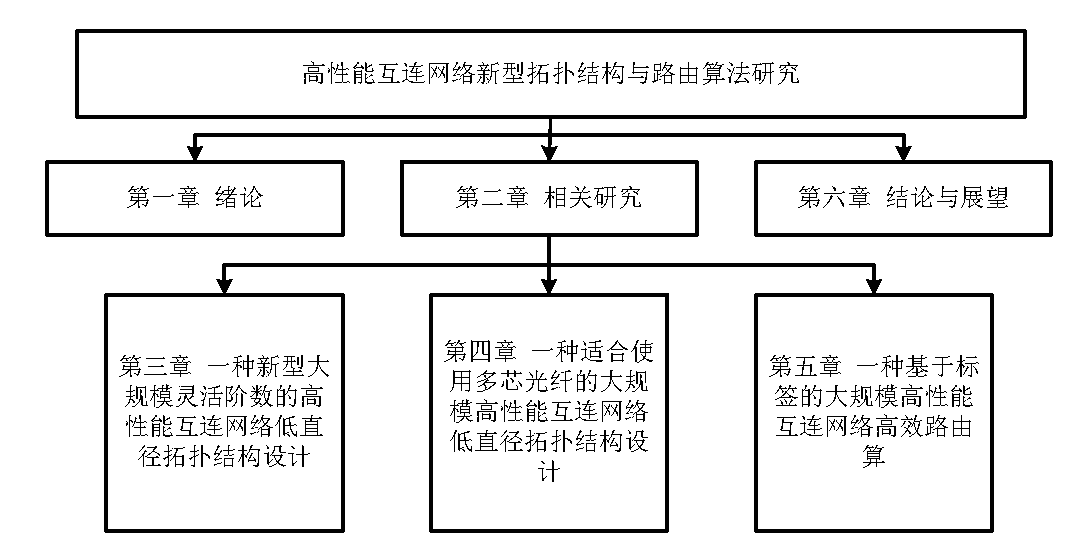
\includegraphics[width=.88\textwidth,height=.45\textwidth]{Visio-org_th.eps}
\caption{论文组织框图}
\label{orgth}
\end{figure}

第一章绪论,首先介绍了高性能计算以及若干典型的高性能计算机系统,
然后论述了高性能互连网络的研究意义以及高性能互连网络设计需要考虑的因素,
然后对高性能互连网络的研究现状以及不足进行了阐述,
最后简述了本文的主要研究内容和组织结构。

第二章介绍了本文的研究背景,包括物理器件对高性能互连网络设计的影响,
最新的高性能互连网络拓扑结构,
高性能互连网络路由算法及高性能互连网络拥塞控制机制。

%%FIXME 用灵活端口数作拓扑结构的定语怪怪的
第三章提出了一种灵活端口数的高性能互连网络低直径拓扑结构Galaxyfly。
首先详细介绍了Galaxyfly拓扑结构的构造方法,
然后对Galaxyfly结构的灵活性、可构造配置、
最短路径数以及容错性进行了详细的理论分析,
之后描述了Galaxyfly结构的路由算法。
最后通过模拟仿真对Galaxyfly的网络性能进行验证。

第四章提出了一种适合采用多芯光纤进行系统部署的高性能互连网络新型拓扑结构Bundlefly。
首先详细介绍了Bundlefly拓扑结构的构造方法,
然后对Bundlefly结构的网络直径、可扩展性、二分带宽、最短路径数、平均最短路径
以及容错性进行了详细的理论分析,
之后描述了Bundlefly结构的路由算法。
最后通过模拟仿真对Bundlefly的网络性能进行验证。

第五章提出了一种基于标签的高性能互连网络路由算法Label-based Routing。
首先详细介绍了Label-based Routing算法的整体架构,
然后描述Label-based Routing算法的缓冲区设计、
路由算法以及虚拟通道分配机制,
最后通过模拟仿真对Label-based Routing的性能进行验证。

第六章结论与展望,对全文的研究内容和主要工作进行总结,并对后续的工作进行展望。
